% !TEX root = ../paper.tex
\section{Interaction techniques} \label{sec:techniques}
In this section we will illustrate and describe the interaction techniques we developed in order to exchange data between mobile phones and large displays.
This is done so that we are capable of comparing them to one another in an emperical way.

There were several criteria behind the choice of these techniques. 
The main one was that users would be able to walk up to a large display and utilize them, which means that they should be as intuitive and natural as possible. 
\cref{tab:techniqueCriteria} shows the set of criteria that we based our choices of techniques on.

\begin{table}[H]
	\centering
	\begin{tabular}{|p{0.2\columnwidth}|p{0.7\columnwidth}|}
		\hline
		\rowcolor[HTML]{9B9B9B} 
		\textbf{Criteria} & \textbf{Description} \\ \hline
		Natural feel & There must be a natural and intuitive feel to the techniques in some way. \\ \hline
		Number of hands & There must be both one-handed and two-handed techniques. \\ \hline
		Previously used & To avoid designing and testing a set of novel techniques, we had the criterion that all techniques must have been used by others before we would use them. \\ \hline
		Complexity & The techniques must differ in their complexity and therefore we included techniques with different amount of steps. \\ \hline
		Activation method & The way each technique is activated must be different from each other. \\ \hline
	\end{tabular}
	\caption{This table describes the set of criteria.}
	\label{tab:techniqueCriteria}
\end{table}
%Two-handed techniques which are techniques that require both hands.


All technique themes were found in the literature.
We then created a mirror version of each technique so they each would have a \push and \pull version.

Eight techniques were chosen in the end: \alltechniques, each with a \push and \pull variant

The \grab techinque is used in \todo{add reference} by Ikemasu et al. as part of an system for exchanging information between different devices. Benko and Wilson \todo{add reference} used the \grab technique in a system were the user would interact with visualizations inside a dome. \grab is a combination of two aformentioned techniques and the pointing technique used by Scheible et al. in \todo{add reference}. This technique was chosen because  

\begin{figure}[H]
	\subfloat[]{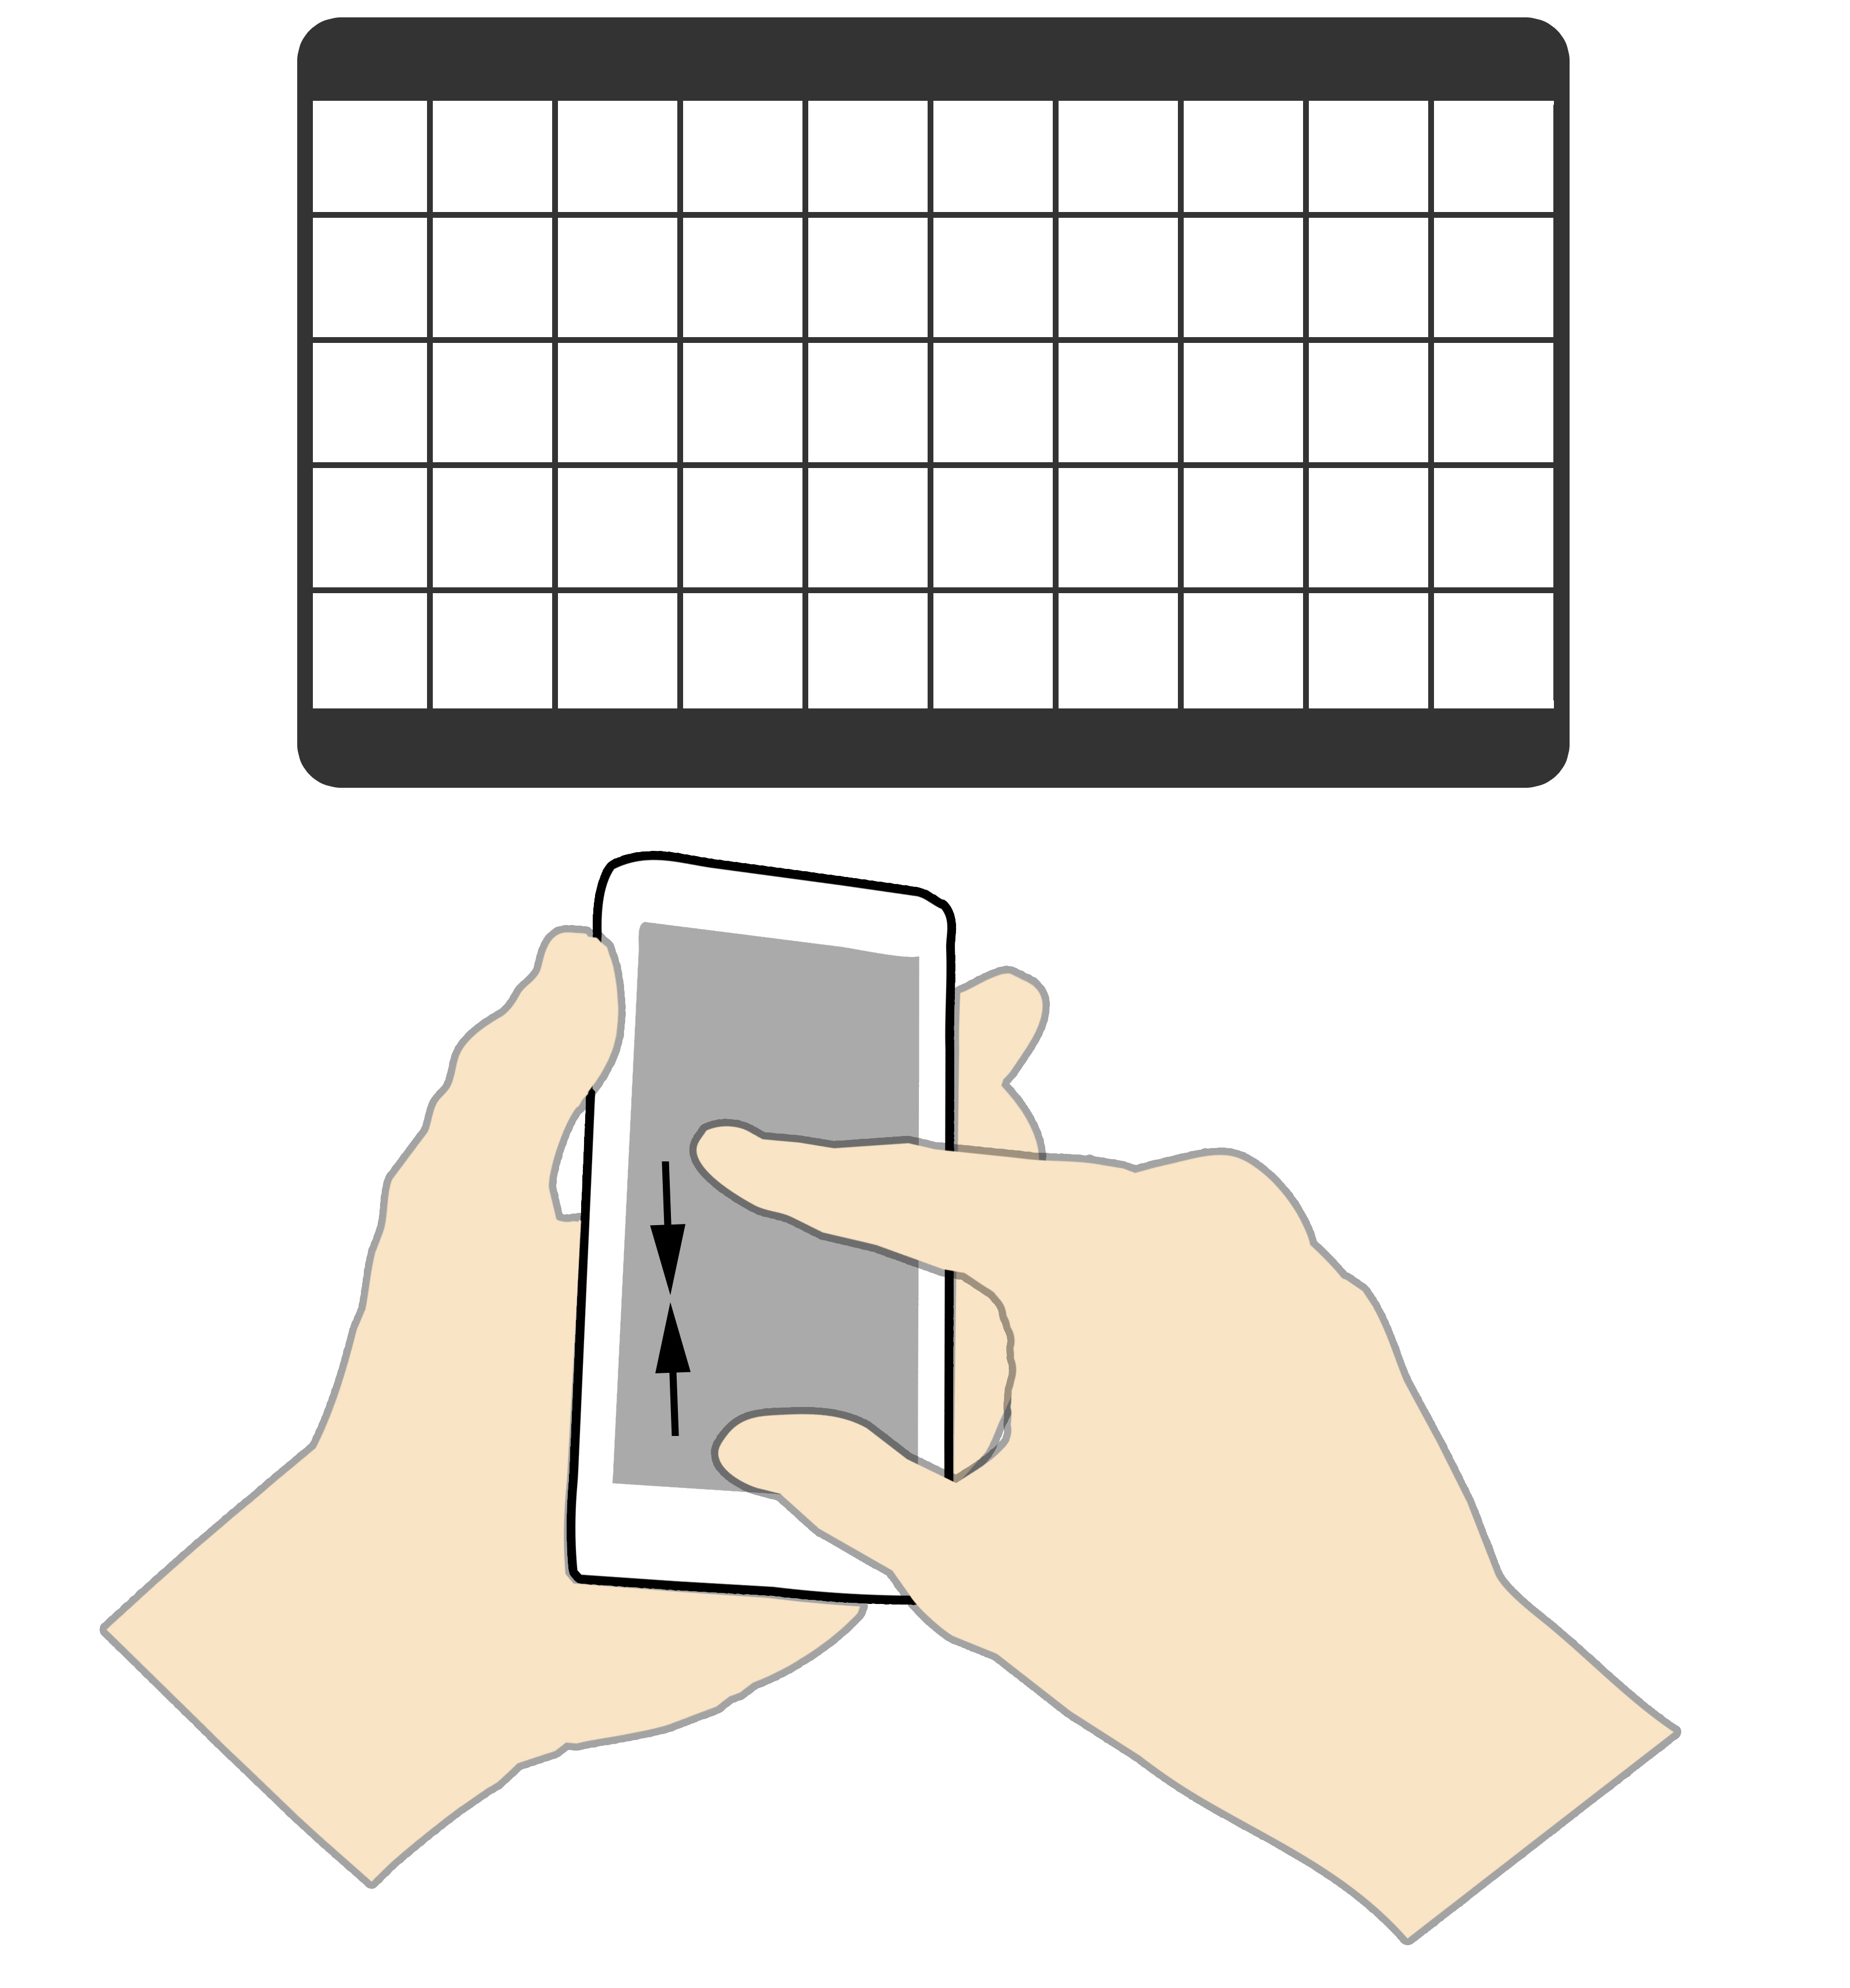
\includegraphics[width = 0.33\columnwidth]{images/pinch_a.jpg}\label{fig:pinchTechniqueA}}
	\subfloat[]{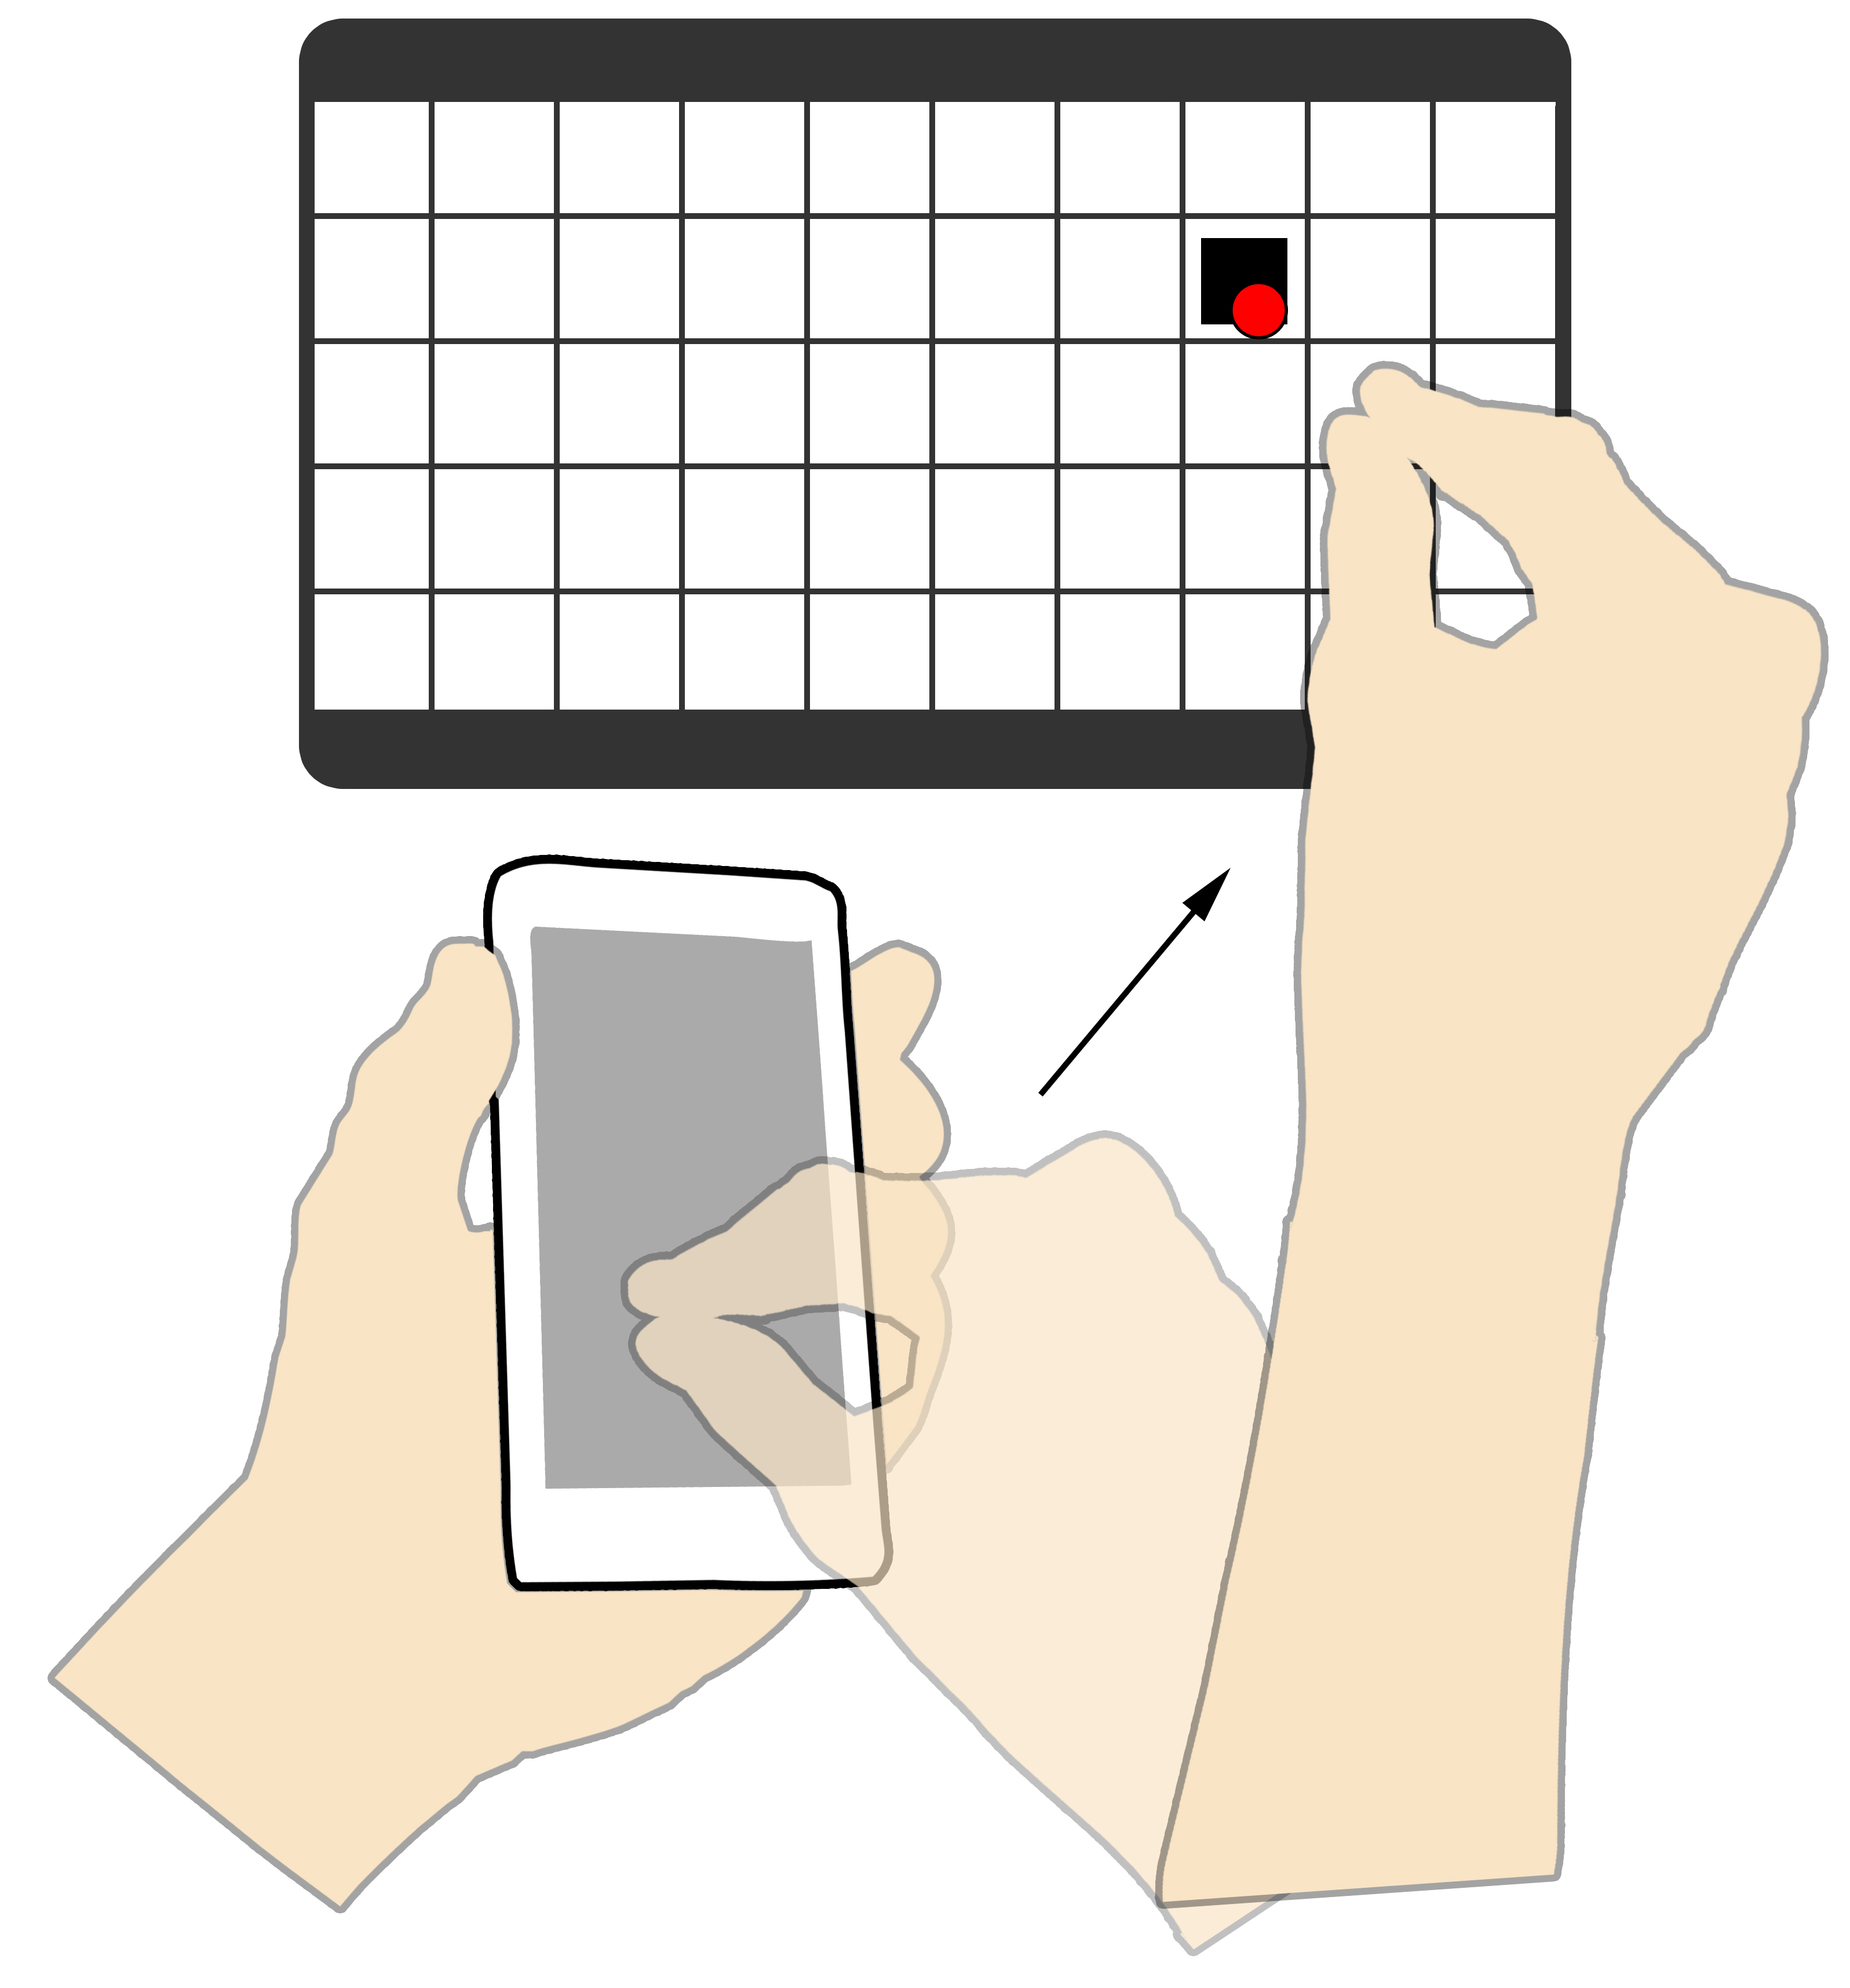
\includegraphics[width = 0.33\columnwidth]{images/pinch_b.jpg}\label{fig:pinchTechniqueB}}
	\subfloat[]{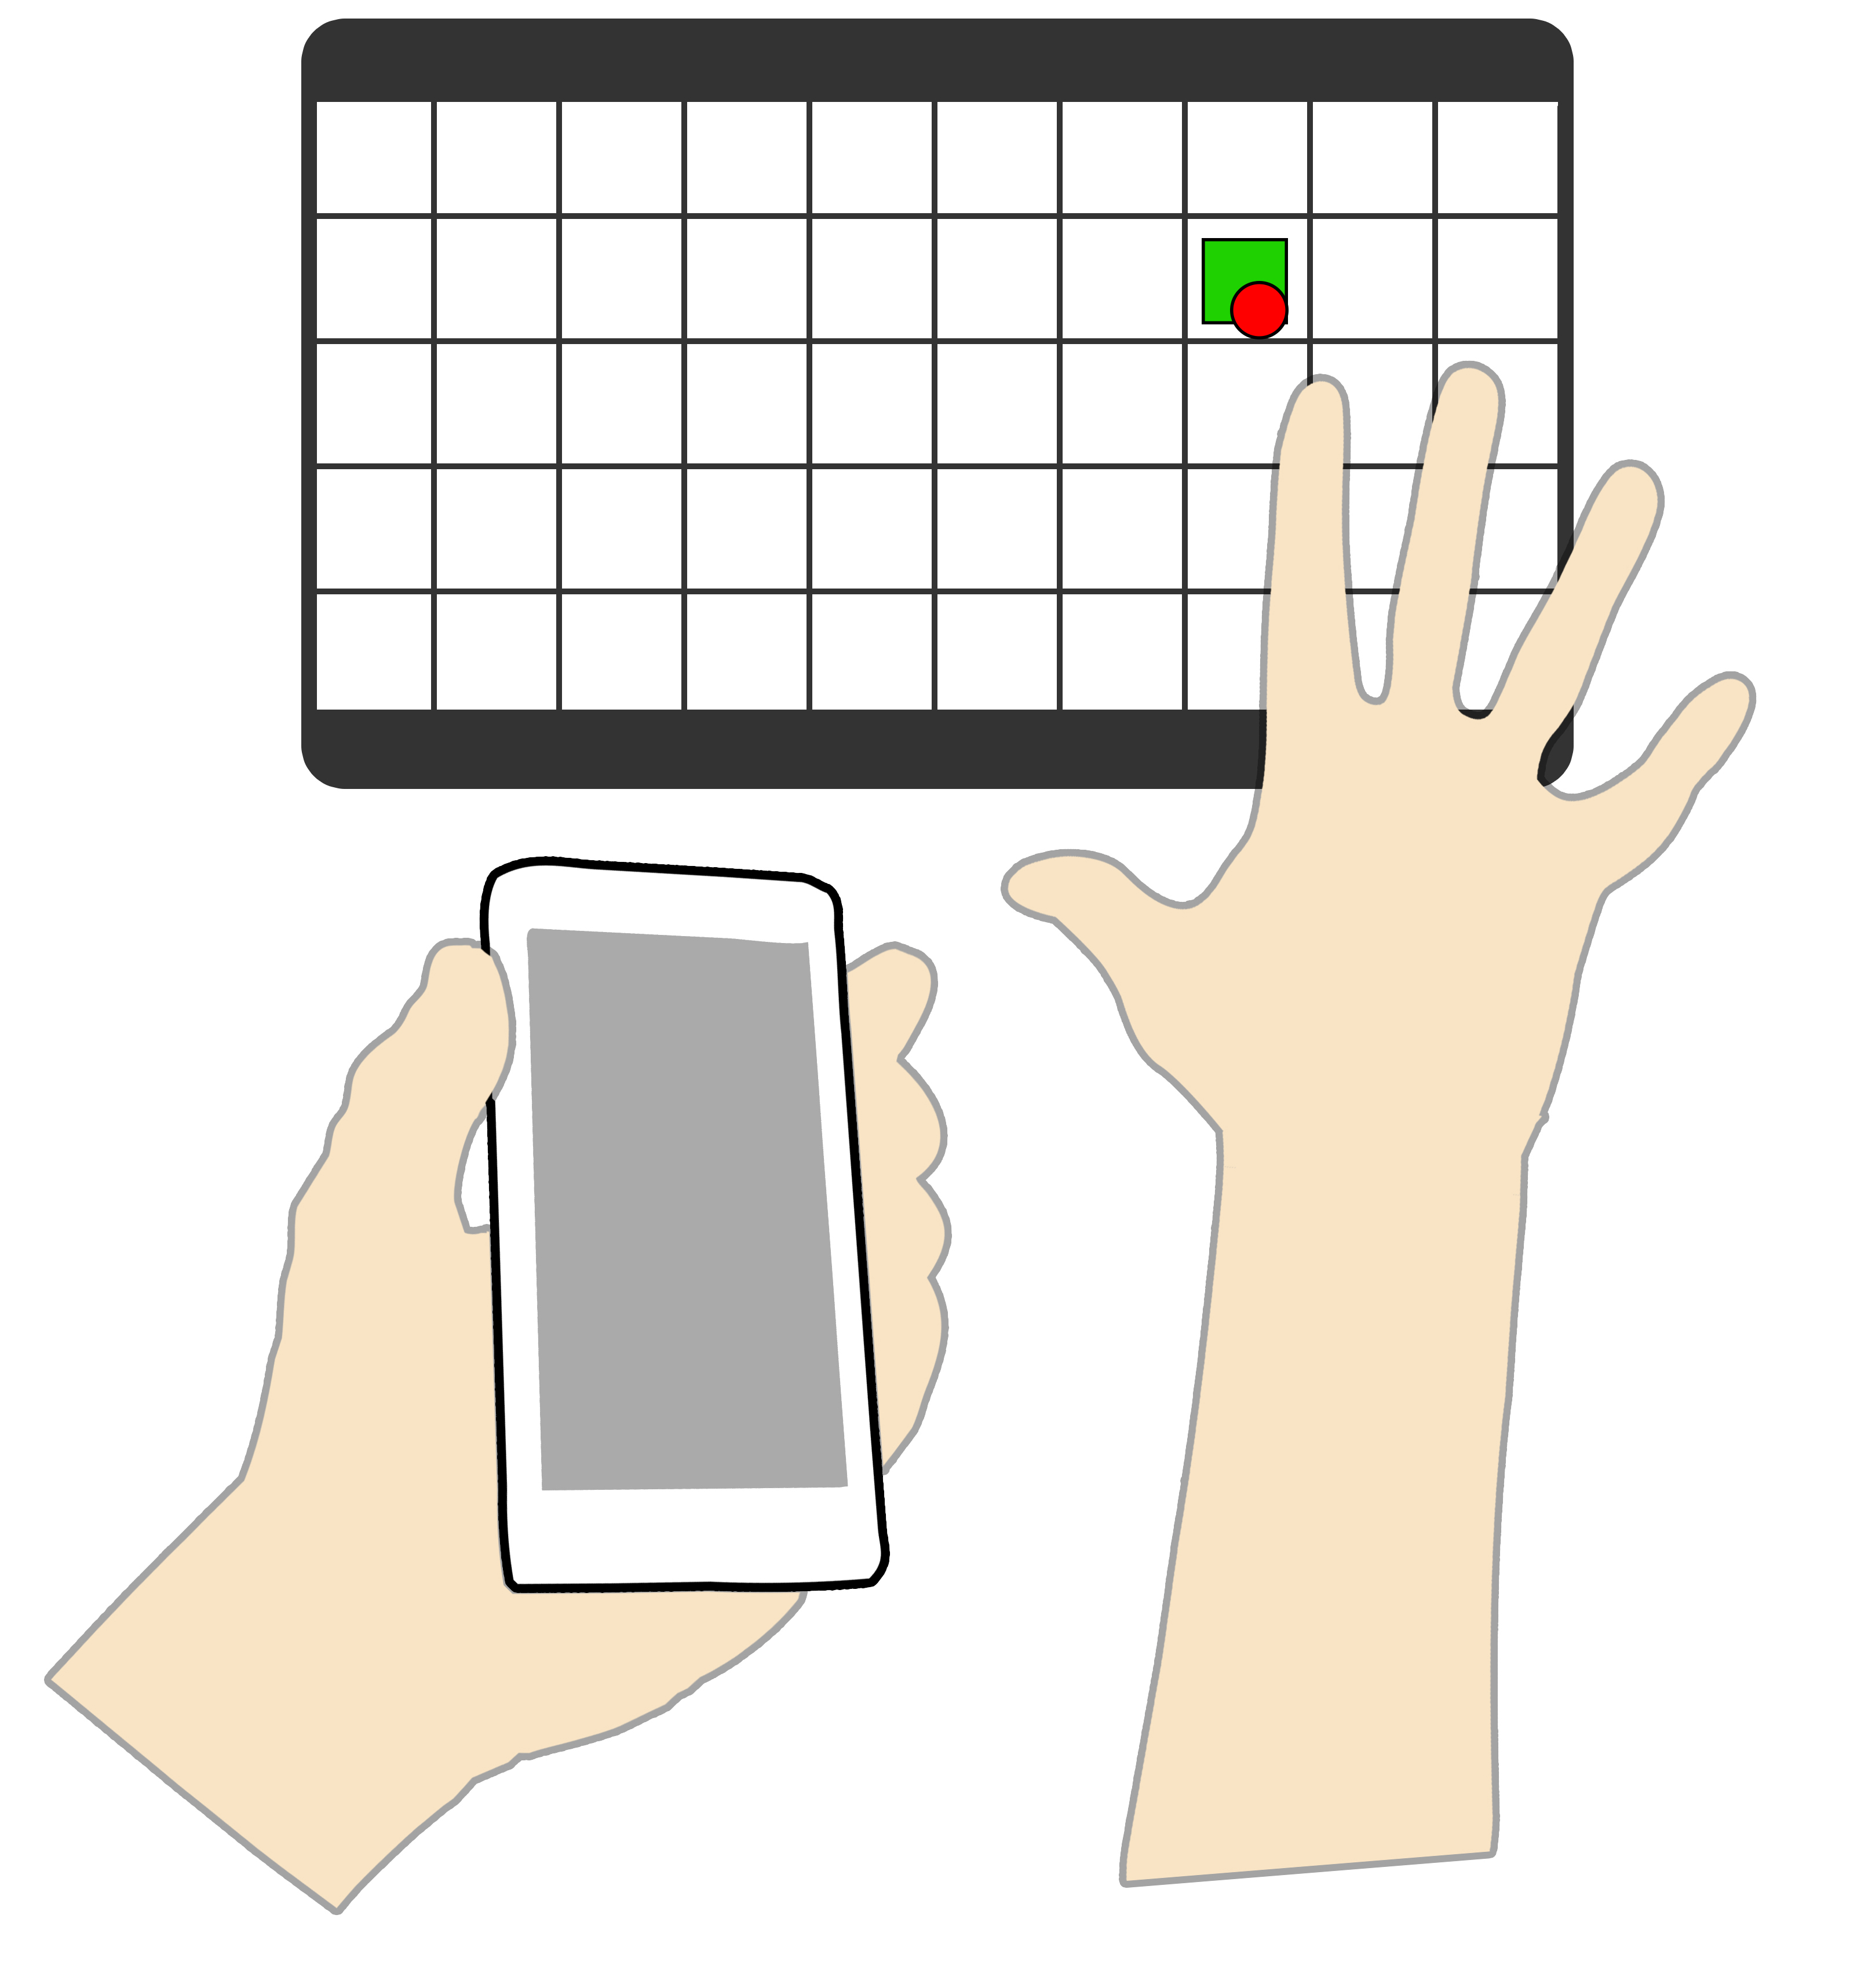
\includegraphics[width = 0.33\columnwidth]{images/pinch_c.jpg}\label{fig:pinchTechniqueC}}
	\caption{\protect\subref{fig:pinchTechniqueA} First step of the \grab technique is to make a grab gesture on the phone by pinching the figure on the phone by using your fingers. \protect\subref{fig:pinchTechniqueB} Second step is to move and use the pinched hand as a pointer. \protect\subref{fig:pinchTechniqueC} Third step is to release by opening the hand.}
	\label{fig:pinchTechnique}
\end{figure}
